\chapter{Hardware Design}
\label{ch:hw_design}
\section{Core Design}
We decided to design and implement two unique RocketCore CPUs for the heterogeneous SoC. These will be in two separate tiles with cache coherency. The aim will be for each core to implement the RV64GC ISA, the 'general-purpose' RISC-V ISA, as well as an MMU (Memory Management Unit) in order to run a full Debian Linux OS, if only with terminal interaction. The following code snippets show the parameterisation options available for the RocketCore CPU and the tiles they lie within.

\begin{figure}
    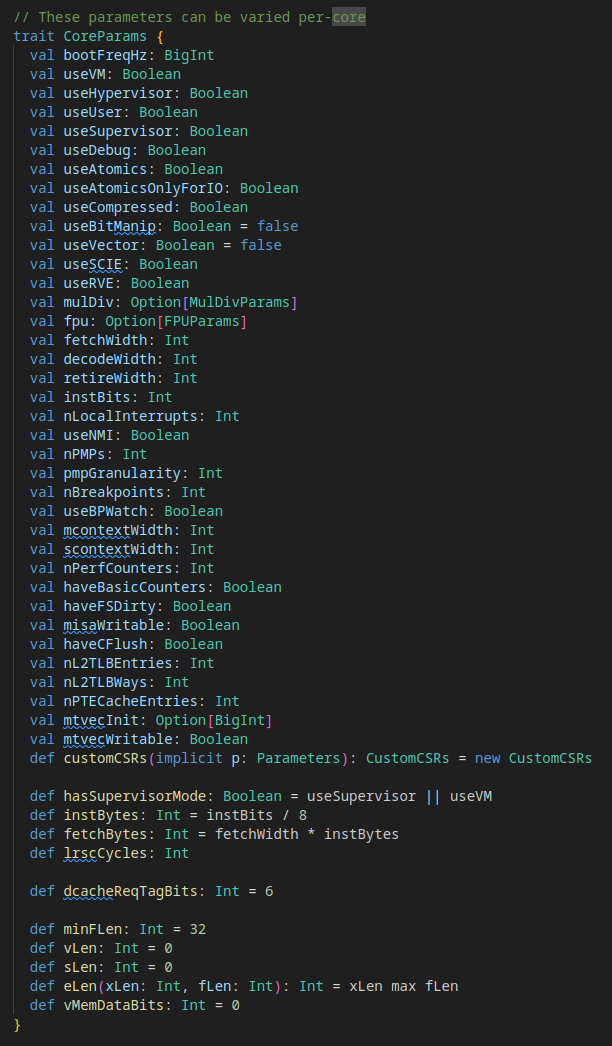
\includegraphics[]{./img/core_params.png}
\end{figure}
\begin{figure}
    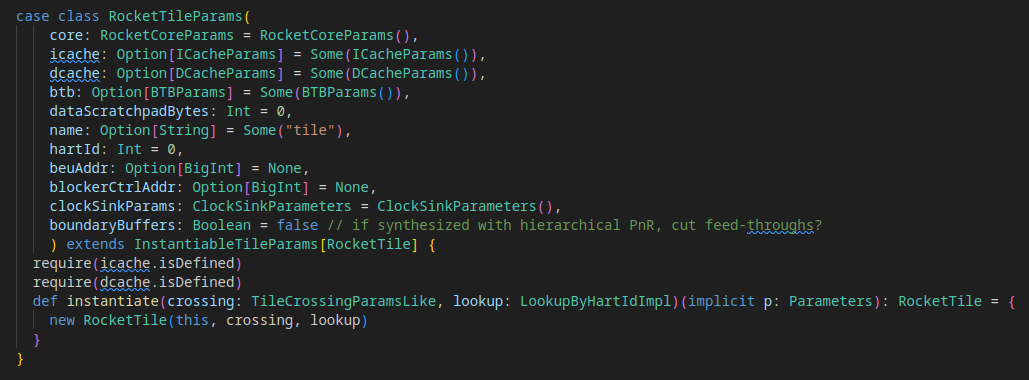
\includegraphics[]{./img/rocket_tile_params.png}
\end{figure}

The micro-architecture specification of RocketCore is not publicised. This means implementation details of the core are not documented, and makes understanding how the core functions a difficult task. For example, to identify what changes occur when \texttt{useVM} is enabled instead of disabled, we must search through the source code (10000+ lines of Chisel in ) to find where the value is used and what it is used for - what other variables are impacted, how they change, etc. 

\subsection{Constant elements in RocketCore}
\subsubsection{Core Frequency - \texttt{bootFreqHz}}
The \texttt{bootFreqHz} core variable does not impact the actual frequency of the core, but instead is added to the device tree structure, so that an operating system is able to read the boot frequency of the CPU. The actual frequency of the cores are defined by clocks generated in the Vivado project. These can be edited, with supported frequencies of 160, 125, 100, 80, 62.5, 50, 40, 31.25, 25, and 20 MHz. The clock manager uses phase locked loop and counters to divide the central clock from the FPGA crystal oscillator. This reduces the available frequencies to those that can be formed from that central clock using the dividers. The Nexys-A7-100t has a crystal capable of generating up to 50 MHz, and is shared between all cores in the RocketChip SoC. This prevents individual clock frequencies for cores, one of the significant changes between big and small cores in typical heterogeneous systems. This will severely limit the actual performance difference between cores, as well as the power consumption difference. This also prevents frequency scaling as the RocketChip SoC does not have control of the clock generator, another key part of modern power saving measures. These are limitations of FPGAs as a platform and the SoC generators used in this project.

\begin{figure}
    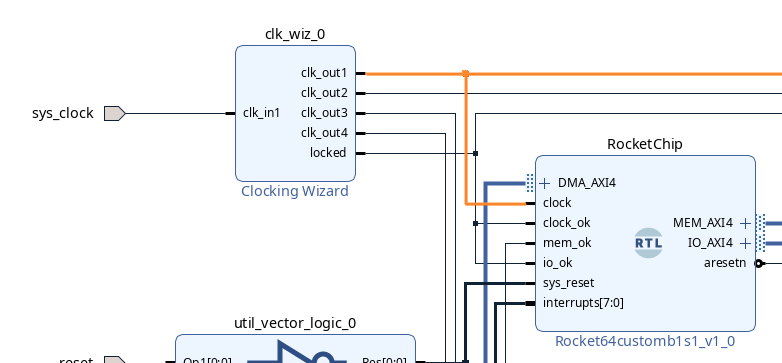
\includegraphics[]{./img/single_clock_rocketchip.png}
\end{figure}

\subsubsection{ALU}
The integer ALU is not customisable within RocketCore. This results in all RocketCore CPUs having the same integer additions per cycle, and as we cannot vary the frequency between cores in the FPGA, all our designs will have the same integer operations per second.

\subsubsection{}

\subsection{MMU - \texttt{useVM}}
The \texttt{useVM} option for core parameters controls whether an MMU (Memory Management Unit) is instantiated inside the core. MMU is enables the use of Virtual Memory, an abstraction of physical addresses to logical addresses. This increases the security and stability of a system, by preventing processes from accessing the memory space of other processes. Stopping reads to another processes' memory space ensures sensitive data currently held in memory by a process cannot be accessed by another process. Stopping writes to the memory space prevents the corruption of another processes' data, that could otherwise lead to user data loss, the process stopping unexpectedly or entire system crash depending on the importance of the memory corrupted process.

The MMU in RocketCore is non-parameterisable - it is either instantiated inside the CPU or it isn't. %todo include LUT comparison with enabled/disabled

\subsection{User/Supervisor modes}
The \texttt{useUser} and \texttt{useSupervisor} options control the addition of hardware privilege levels. All RISC-V CPUs have the machine privilege level (M-mode). Code run in M-mode is able to execute any instruction, including those that would result in the CPU becoming trapped permanently. M-mode is intended to be used for managing secure execution done in lower privilege levels, completely trusted code that must be run on M-mode for system setup or for embedded systems where M-mode is the only privilege level implemented.

User mode (U-mode) can be added to the CPU to provide a secure environment where code can be executed safely, and wouldn't be able to cause serious damage to the system. The CPU keeps track of state at prevents this, but current privilege level is not visible to software as this would become a virtualisation hole - a way for a program to attempt to escape or see outside it's current virtualisation level. Privileged instructions cannot be run in U-mode, preventing access to registers such as \texttt{mtvec}, keeping the address of the machine trap vector and mode. U-mode is typically implemented for secure embedded systems, where a level of privilege is required to ensure the system does not fail when application code is run.

Supervisor mode (S-mode) can also be added. This privilege level fits between U-mode and M-mode, adding many S-mode registers that only M-mode had previously, such as \texttt{SPP} for the previous privilege mode or \texttt{stvec} for the supervisor trap vector address and mode. S-mode is utilised most often by OSs that want to be able to run applications on top of themselves and keep functioning, so must prevent such applications from being able to maliciously or accidentally interfere with it's operation.

As the SoC designed by this project will never be put into a production environment, we can remove user and supervisor modes, executing all programs in machine mode. While this removes all hardware security from the system, the only code being run will be either written by the author or from trusted open-source projects. In addition to this, the system is completely isolated and would be unable to cause any damage if compromised, only connected to another system via serial.

\subsection{Hypervisor mode}
\texttt{useHypervisor} option enables the hypervisor mode extension. Hypervisor mode extends supervisor mode, adding additional virtualisation. S-mode becomes HS-mode, where a hypervisor program or hosting-capable OS runs, and changes some registers typically accessed from \texttt{Sxxx} to \texttt{Hxxx}, such as \texttt{SIE} to \texttt{HIE}. A virtualisation bit is added and set when the CPU is executing a guest OS, and this changes the HS-mode and U-mode to VS-mode and VU-mode. An additional layer of address translation is enabled when this occurs, as well as the registers accessed in VS-mode returning to the \texttt{Sxxx} versions.

This mode is used for systems where multiple OSs may be running concurrently, such as servers or workstation PCs. This project does not aim to design an SoC to be used in this context and we can safely disable this option.

\subsection{Debug mode}
Debug mode has been preliminarily proposed as an extension to the RISC-V ISA. The \texttt{useDebug} option controls the implementation of this extension. When enabled, this generates hardware in the core to enable debugger control of the core, as well as a debugger module in the SoC. The changes to the core include addition of CSR registers, writable only by an external debugger interacting with the debug module, that can halt execution, force jumps, and other control functions. The debug module allows an external debugger to get the contents of core data registers, cache, RAM, and CSRs as needed, enabling someone testing hardware to inspect the status of the core during program execution. The debug module also provides the capability to 'step through' the instructions, a very useful feature when identifying the exact instruction where a program deviates from expected execution.

We have enabled this option during the design phase, as the debug features it provides is very useful when designing the test software. For the actual core under test the option was disabled, to reduce the FPGA usage for comparisons and maximise the available resources for additional processing hardware.

\subsection{Atomics}
The \texttt{useAtomics} and \texttt{useAtomicsOnlyForIO} options enable parts of the Atomic RISC-V extension. The atomic extension implements instructions allowing for read-modify-write to memory and IO while keeping memory consistency between multiple RISC-V harts utilising the same memory/IO.

Base RISC-V ISA has a relaxed memory model, allowing loads and stores to take place in any order if unspecified. The atomic extension implements load-reserved and store-conditional instructions that can apply additional ordering constraints on memory/IO operations, and ensure data is valid during operations performed on it. There are two bits used to specify acquire and release ordering requirements for this RISC-V hart: when the acquire bit is set, no memory operation instructions following the acquire-set instruction can take place before the acquire-set operation; when the release bit is set, the release-set instruction must take place after any previously issued memory operations. The combination of these bits allow for sequential ordering of memory operations for a RISC-V hart can be asserted. These instructions are primarily utilised for out-of-order CPUs, where the ordering of issued instructions does not necessarily match the order of instruction execution, leading to race conditions without atomically defined instructions.

The atomics also implement instructions for multicore synchronisation. Atomic write-modify instructions for memory perform changes that occur uninterrupted with a single instruction. These also implement the acquire and release bits, and allow for swapping, addition, bitwise operations and maximum/minimum instructions to be completed on data held in shared memory without other harts interefering.

As the system we are designing is multicore, we enabled the \texttt{useAtomics} option. Not allowing simultaneous memory access in a multicore system would cause a severe bottleneck in most cases and is the only other solution to ensure memory validity in this case.

\subsection{Compressed instructions}
Enabling the compressed instruction set extension is done using the \texttt{useCompressed} option.

\subsection{Default RocketCore CPUs}
RocketCore contains some predefined core designs. These allow a user to immediately generate a RocketCore CPU without having to parameterise their own, with a few different options dependant on the use case.

\subsubsection{Small Core}
The RocketCore predefined small core implements the RV64IMAZicsrZifenceiC ISA, removing the single-precision floating point and double-precision floating point instructions from the RV64GC ISA. The point of this is to remove the FPU from the CPU, much reducing the logic required by the design.

\begin{figure}
    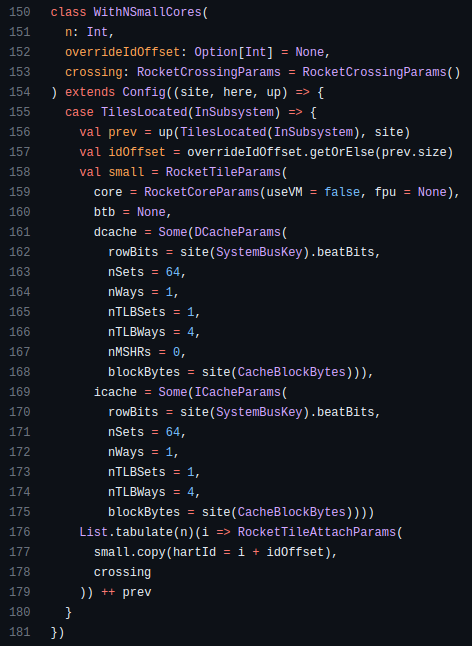
\includegraphics[]{./img/rocketcore_default_small.png}
\end{figure}

The MMU has also been removed from the CPU, preventing virtual memory from being used. The removal of virtual memory allows programs to interfere with each others memory, and this can be very difficult to deal with if programs are dynamic in memory and the amount of memory they consume. The main issues stemming from this are lack of security and instability. Virtual memory invalidates read attempts to memory spaces not under the control of that process, and no virtual memory allows a malicious process to read any other processes memory, including any sensitive data they might hold. Virtual memory also prevents write attempts to other processes memory space, and so a process might overwrite another's memory during runtime, leading to one process, both processes or the entire system stopping unexpectedly.

The core has separate data and instructions caches, each with 64 sets of 1 ways, giving 64 lines of 8 bytes and a total of 512 bytes. This is a very small, and any computation that uses many pieces of data will be very memory bound.

A small BTB (Branch Target Buffer) with 28 entries and a BHT (Branch History Table). The BTB stores the destination of recent branches, with the BHT the history of whether the branch was taken. This forms a branch predictor, that attempts to predict if a branch is taken and if so, where it will jump to. This is a relatively small branch predictor, and would suffer in complex programs with many varying branches.

The multiplier divider unit is small, without unrolling or early out. 

\chapter{Test Design}
\label{ch:test_design}

\section{Software Verification}
Software verification was completed using the Spike RISC-V emulator. Spike is a functional model of a RISC-V processor, with options for number of harts (hardware threads, RISC-V representation of logical cores), and ISA. Spike supports all major ratified extensions, as well as some still in the proposed stage. As our final hardware implementation uses RV64IMAZicsrZifenceiC, we can set Spike to simulate the same core type when invoking from the command line.

